\chapter{Uczenie} 
{
    Do przetworzenia danych do wybranej postaci, również zostały wykorzystane modele wymagające uczenia.
    Pierwszym z opisanych nich jest model k-Means, który został wykorzystany w celu wyznaczenia klastrów
    długości trwania dźwięków. Do głównych parametrów tego modelu należy docelowa ilość klastrów, ilość iteracji
    oraz niezależnych uruchomień modelu mające na celu rozwiązania problemu zatrzymywania uczenia w lokalnym minimum.
    
    Kolejnym zastosowaniem uczenia maszynowego w etapie przetwarzania danych było użycie algorytmu Word2Vec. Algorytm 
    został użyty do wyznaczenia ciągłej reprezentacji rzadkich wektorów reprezentujących dźwięki. Model wymagał 
    określenia docelowej wymiarowości wektorów i rozmiaru kontekstu. 

    W poniższych podrozdziałach skupiono się jednak na uczeniu głównego modelu, czyli sieci neuronowej której
    zadaniem jest ekstrakcja cech utworów treningowych.

    \section{Architektura modelu}
    {
        Otrzymawszy dane w postaci sekwencji par wektorów opisujących dźwięki i ich czas trwania,
        przystąpiono do projektu architektury modelu. Z powodu dwuelementowej postaci danych
        zdecydowano się na zaprojektowanie modelu dwuwejściowego i dwuwyjściowego.

        Ponieważ charakter wektorów w sekwencji jest różny - wartości ciągłe opisujące dźwięki i 
        kategoryczny kod 1 z N opisujący długość dźwięku - przed złączeniem wektorów postanowiono 
        przekształcić wektor 1 z N przez warstwę gęstą o wymiarze mniejszym niż N. Celem tej operacji
        było wprowadzenie konieczności przez sieć kompresji informacji, co najprawdopodobniej przełoży się 
        na wyznaczenie ciągłej reprezentacji kodu o mniejszej wymiarowości. 

        Następnie wektory zostają złączone, i ich sekwencje trafiają do warstw rekurencyjnej sieci LSTM,
        w której model ma szanse ekstrahować wiedzę o zależnościach między elementami sekwencji.

        Otrzymywane wektory są połączone do osobnych, mniejszych sieci LSTM i następnie poprzez warstwy 
        gęsto połączone stają się osobnymi wyjściami modelu.
        
        Wyjście odpowiedzialne za dźwięki uczone jest funkcją błędu odpowiednią do problemu 
        regresji - błędem średniokwadratowym, a wyjście klasyfikujące długość dźwięku funkcją odpowiednią
        dla zadania klasyfikacji 1 z N - categorical crossentrophy.
    }

    \section{Dobór parametrów}
    {
        Podczas procesu uczenia najistotniejszymi parametrami były:
        \begin{itemize}
            \item rozmiar okna, czyli długość uczonych sekwencji,
            \item ilość przykładów w wiązce, czyli ile sekwencji było uczonych jednocześnie
            poprzedzając pojedyncze przeprowadzenie algorytmu propagacji wstecznej,
            \item rozmiar głównej sieci LSTM.
        \end{itemize}
    }

    \section{Proces uczenia}
    {
        Podczas uczenia modelu zdecydowano się na dynamiczny rozmiar okna,
        będący liczbą losową z zakresu <15, 50>. Motywacją tego wyboru były testowe 
        uruchomienia modelu potwierdzające zdroworozsądkową intuicję mówiącą, że większe wartości
        umożliwią uczenie dłuższych powtarzających się motywów, a krótsze lokalne następstwo nut.

        Dodatkowo, warto przybliżyć sposób tworzenia przypadków testowych. Naiwnym podejściem byłoby
        jednokrotne utworzenie zbioru danych poprzez utworzenie wszystkich możliwych podciągów o zadanej
        długości (rozmiarze okna) i dalsze używanie ich jako statycznej listy przypadków. 
        Takie rozwiązanie nie umożliwiałoby dynamicznej zmiany długości sekwencji, i wymagałoby dodatkowego 
        kroku w procesie przetwarzania danych. Alternatywnym podejściem, na które się zdecydowano jest dynamiczne
        wybieranie losowych podciągów z utworów należących do zbioru danych, które odbywa się równolegle z uczeniem modelu. 
        Główną obawą jaką można posiadać do takiego podejścia jest jego narzut podczas uczenia modelu, 
        aczkolwiek zaobserwowano że tempo przygotowania i kolejkowania kolejnych przypadków testowych znacznie przewyższa tempo ich uczenia.

        Podczas testowania różnych wartości innych parametrów, zaobserwowano Interesujący wpływ ilości przykładów w wiązce.
        %%% można jakby co opisać czym jest wiązka 
        Większe wartości, rzędu 16 lub 32 miały negatywny wpływ na jakość generowanych sekwencji. 
        Mniejsze wartości prowadziły do przetrenowania modelu.

        Rozmiar głównej sieci miał spodziewany efekt, nieodpowiednio duży prowadził do przetrenowania. Dla obecnego
        zbioru danych zdecydowano się zachować wartość 64 jednostek.

        Podczas uczenia monitorowano metryki opisujące jakość predykcji i postęp uczenia modelu.
        Do mierzonych metryk należą funkcje błędu dla poszczególnych wyjść modelu, średni błąd kwadratowy
        wyjścia reprezentującego wektory dźwięków oraz kategoryczna dokładność stwierdzająca czy najwyższa wartość
        wektorów znajduje się na tym samym indeksie.
        
        Uczenie podzielone było na epoki. W klasycznych zastosowaniach przez jedną epokę rozumie się jednokrotne
        wykorzystanie każdego przykładu z zbioru treningowego. Jednakże z powodu opisanego powyżej sposobu otrzymywania
        przypadków testowych, niemożliwe było wykorzystanie tej definicji. Zdecydowano się na arbitralne przyjęcie konkretnej 
        ilości przypadków testowych jako jednostkę jednej epoki. Obraną wartością był tysiąc.

        Po ukończeniu każdej epoki przeprowadzane były pomiary skuteczności modelu na danych wyjętych spoza korpusu 
        danych treningowych. Ponieważ problematycznym byłoby wydzielenie sekwencji walidacyjnych z części środkowych
        utworów, zdecydowano się zarezerwowanie ostatnich 25 elementów sekwencji z każdego utworu.
        Na podstawie powyższych wyników, można wyciągać wnioski dotyczące postępu uczenia modelu.

        Uczenie zaplanowano na okres 35 epok, co przełożyło się na czas bliski 20 minut. Do uczenia wykorzystano
        akcelerację sprzętową w postaci karty graficznej dostępnej w usłudze chmury obliczeniowej Google Colab.

        Ilustracje \ref{epoch_val_duration_output_categorical_accuracy} i \ref{epoch_val_notes_output_mean_squared_error} zawierają wykresy opisujące miary postępu uczenia podczas kroków walidacyjnych.

        \begin{figure}
            \centering
            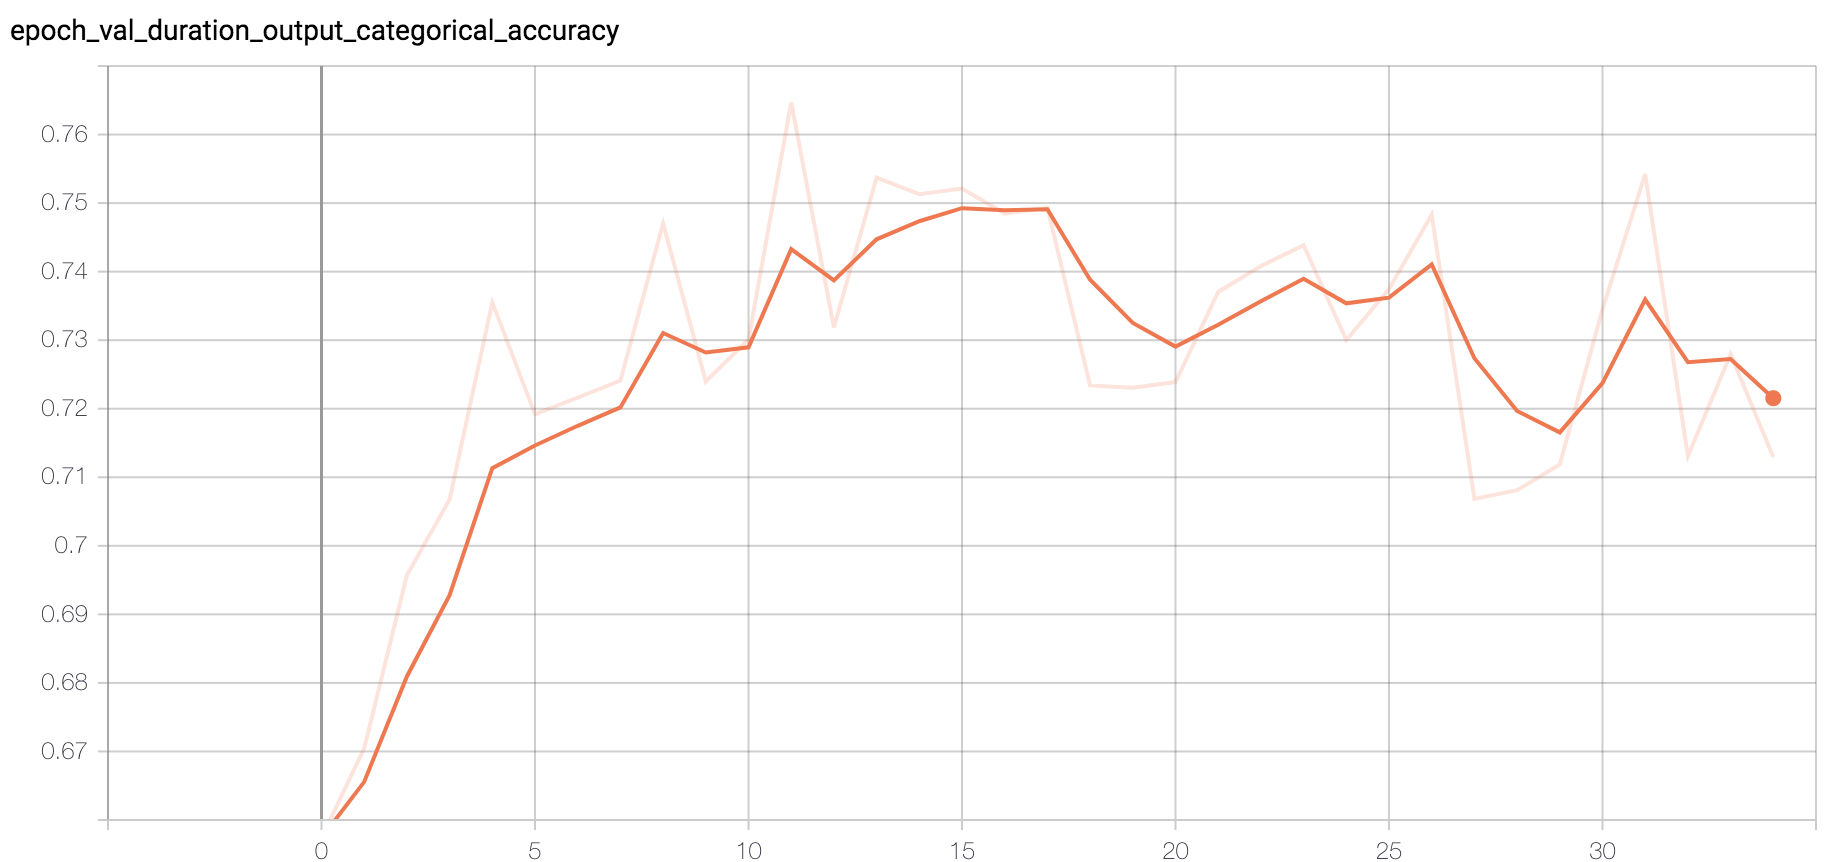
\includegraphics[scale=0.4]{epoch_val_duration_output_categorical_accuracy}
            \caption{Wartości miary precyzji predykcji długości trwania dźwięków}
            \label{epoch_val_duration_output_categorical_accuracy}
        \end{figure}
        
        \begin{figure}
            \centering
            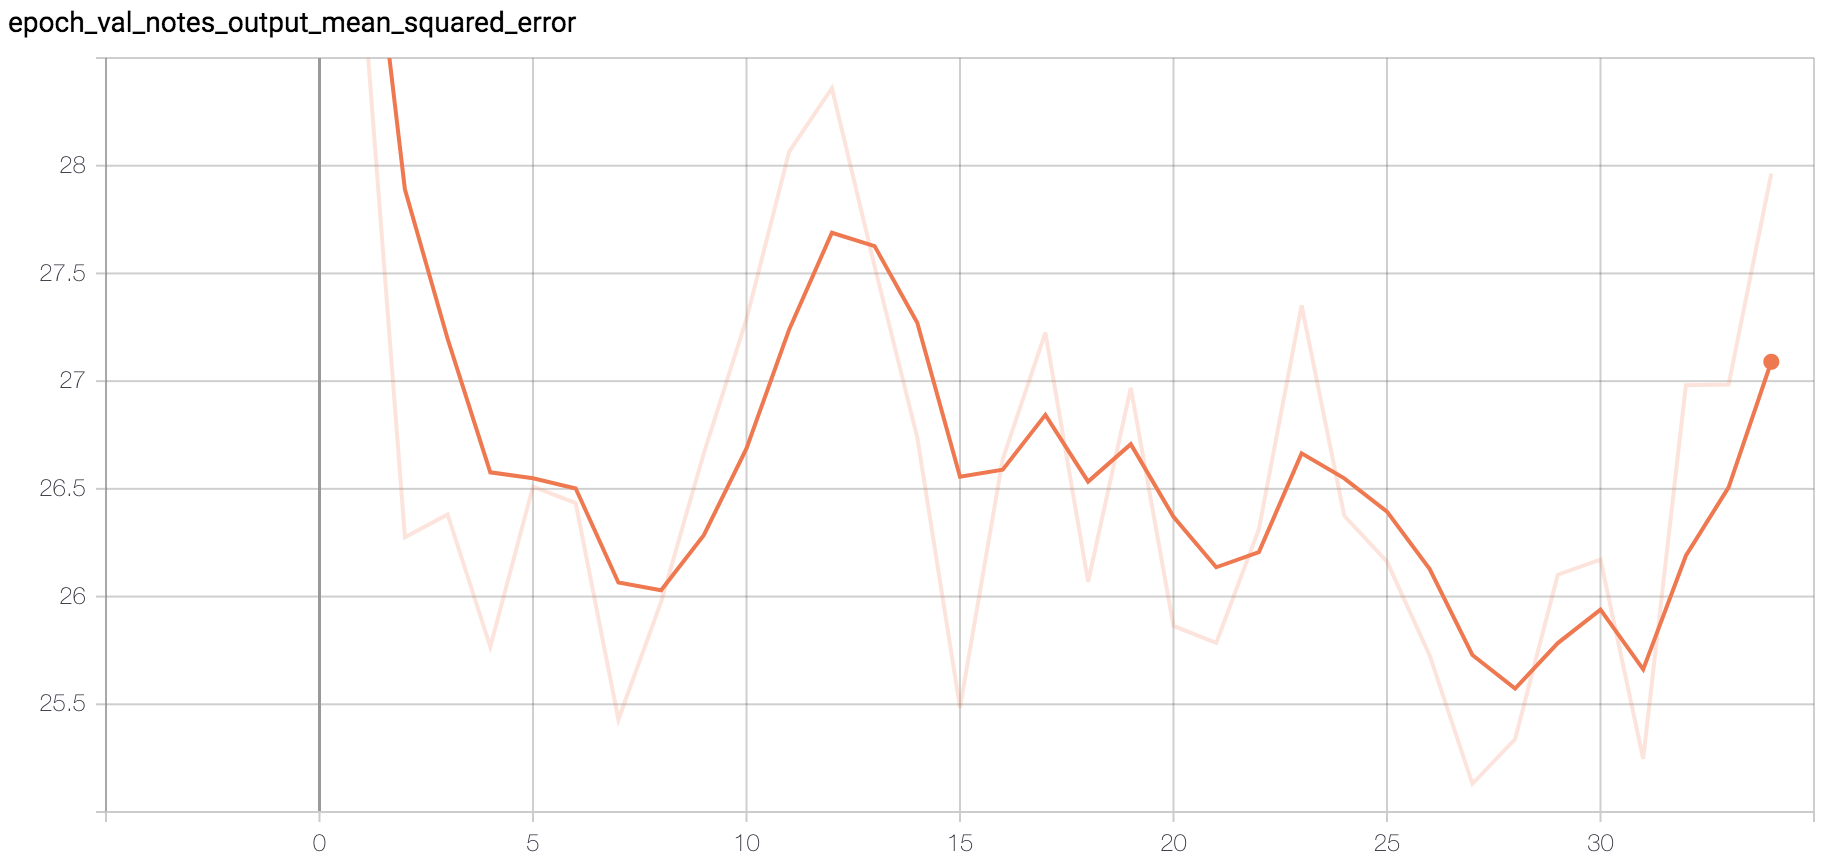
\includegraphics[scale=0.4]{epoch_val_notes_output_mean_squared_error}
            \caption{Wartości błędu średniokwadratowego predykcji wektora dźwięków}
            \label{epoch_val_notes_output_mean_squared_error}
        \end{figure}

        Na ilustracjach można dostrzec trafność predykcji klasy długości trwania dźwięku, oraz błąd średniokwadratowy
        predykcji wektorów dźwięków. W pierwszej połowie uczenia na obydwu wykresach można zaobserwować pożądaną tendencję,
        czyli wzrost trafności i spadek błędu. Po kolejnych epokach postęp uczenia malał, lub nawet zachodził jego regres.
    }
}